\subsection{Exercises}

%%%%%%%%%%%%%%%%%%%%%%%%%%%%%%
\Large{Problem 3.1}
\begin{figure}[H]
    \centering
    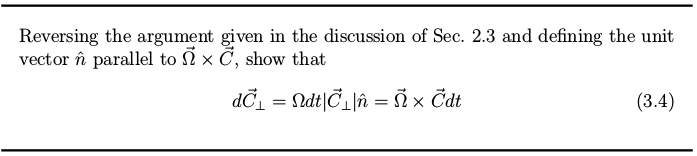
\includegraphics[width=0.8\textwidth,keepaspectratio]{prbl31}
    \label{fig:prbl31}
\end{figure}

\textit{Remember:}
\begin{itemize}
	\item The perpendicular component (perpendicular to $\vec{\Omega}$, 
	the rotational angular velocity vector of the rotating frame) of some vector $\vec{C}$ at rest in 
	the rotating frame has a differential change whose magnitude can 
	be calculated.
	\item The parallel component does not change through time.
    \item $\vec{\Omega} \times \vec{C} $ = anti-clockwise rotation 
\end{itemize}

\textit{Proof.}
\begin{flalign*}
    \frac{d\vec{C}}{dt} &= \vec{\Omega} \times \vec{C} \\
    \frac{d(\vec{C}_{\perp} + \vec{C}_{\|})}{dt} &= \vec{\Omega} \times (\vec{C}_{\perp} + \vec{C}_{\|}) \\
    \frac{d\vec{C}_{\perp}}{dt} + \frac{d\vec{C}_{\|}}{dt} &= \vec{\Omega} \times \vec{C}_{\perp} + \vec{\Omega} \times \vec{C}_{\|} \\
    \frac{d\vec{C}_{\|}}{dt} &= \vec{\Omega} \times \vec{C}_{\|} \\
                             &= \Omega \, \lvert \vec{C_{\|}} \rvert \, sin \,
    0^o \, \hat{n} = \mathbf{0} \\
                             & \Rightarrow \\
    \frac{d\vec{C}_{\perp}}{dt} &= \vec{\Omega} \times \vec{C}_{\perp} \\
    d\vec{C}_{\perp} &= \Omega\, dt \lvert\vec{C}_{\perp}\rvert\, sin \theta\, \hat{n} \\
    \text{But} \, \theta = 90^o &\Rightarrow sin \, \theta = 1 \Rightarrow \\
    d\vec{C}_{\perp} &= \Omega\, dt \lvert\vec{C}_{\perp}\rvert\, \hat{n}
\end{flalign*}

\clearpage
%%%%%%%%%%%%%%%%%%%%%%%%%%%%%%
\Large{Problem 3.2}
\begin{figure}[H]
    \centering
    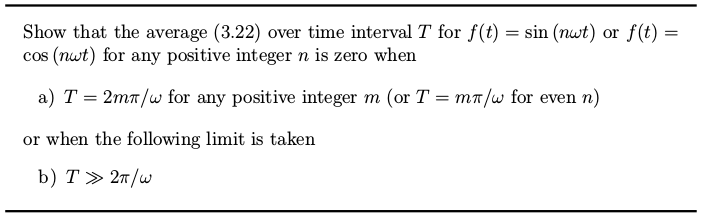
\includegraphics[width=0.8\textwidth,keepaspectratio]{prbl32}
    \label{fig:prbl32}
\end{figure}

\textit{Remember:}
\begin{itemize}
	\item In the rotating reference frame, only half of the original 
	linearly polarized field ($\vec{B_1}^{lin} = b_1^{lin} \, cos \, 
	(\omega t) \, \hat{x}$) is available to tip the spin ($\vec{B_1}^{lin} = 
	\frac{1}{2} \, b_1^{lin} [\hat{x}' (1 + cos \, 2 \omega t) + 
	\hat{y}' sin \, 2 \omega t]$).
	\item The idea is that the effects of the oscillating terms 
	average to zero over times that are half multiples of the rf 
	period, or for all times large compared to the rf period.
\end{itemize}

\textit{Also remember:}
\begin{align*}
    \int_{0}^{2 \pi} sin(x) dx = 0 \\
    \int_{0}^{2 \pi} cos(x) dx = 0 \\ 
    \int_{\frac{- \pi}{2}}^{\frac{\pi}{2}} cos(x) dx = 2 \\
    \int_{0}^{\pi} sin(x) dx = 2 
\end{align*}

\textit{a) Proof.}
\begin{flalign*}
    <f(t)>\, \equiv \frac{1}{T} \int_0^T f(t) dt &= \frac{1}{T} \int_0^T sin(n\omega t) dt \\
                                 &= \frac{\omega}{2m\pi} \int_0^{\frac{2m\pi}{\omega}} sin(n\omega t) dt \\
                                 &= \frac{\omega}{2m\pi} [-cos(n \omega t) \frac{1}{n\omega}]_{0}^{\frac{2m\pi}{\omega}} \\
                                 &= \frac{1}{2nm\pi} (-cos(2nm\pi) + cos(0)) \\ 
                                 &= \frac{1}{2nm\pi} - \frac{1}{2nm\pi} cos(2nm\pi) \\
    \text{We know that: } cos(2N\pi) &= 1 \text{ for } N \in \mathbb{Z} \Rightarrow \\
    \frac{1}{T} \int_0^T f(t) dt &= 0 
\end{flalign*}

\textit{b) Proof.}
\begin{flalign*}
    <f(t)>\, \equiv \frac{1}{T} \int_0^T f(t) dt &= \frac{1}{T} \int_0^T sin(n\omega t) dt \\
                                                 &= \frac{1}{T} [-cos(n\omega t) \frac{1}{n \omega}]_{0}^{T} \\
                                 &= \frac{1}{n \omega T} (- cos(n \omega T) + cos(0)) \\
                                 &= \frac{1}{n \omega T} (1 - cos(n \omega T)) \\
\end{flalign*}



%\begin{figure}[H]
%    \centering
%    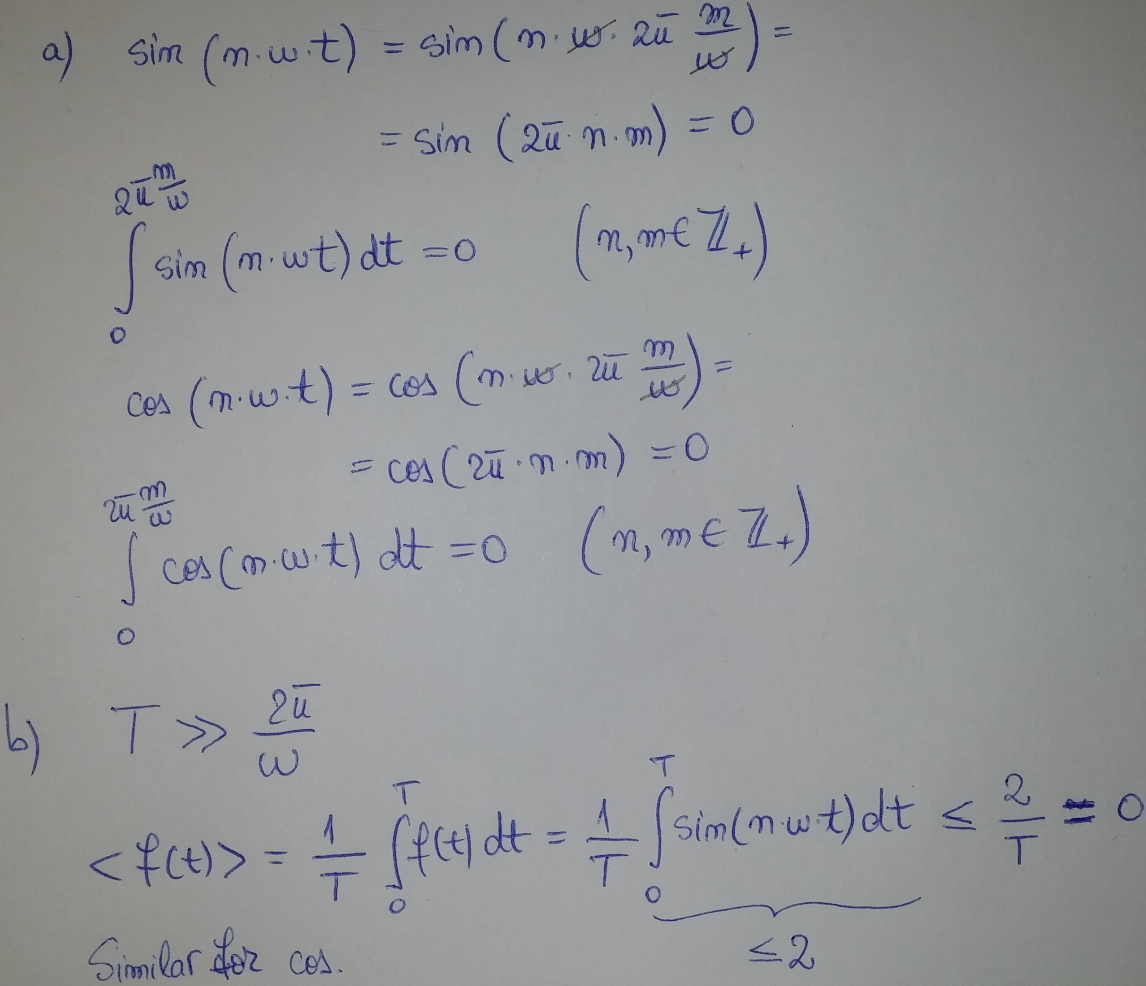
\includegraphics[width=0.8\textwidth,keepaspectratio]{prbl32s}
%    \label{fig:prbl32s}
%\end{figure}

\clearpage
%%%%%%%%%%%%%%%%%%%%%%%%%%%%%%
\Large{Problem 3.3}
\begin{figure}[H]
    \centering
    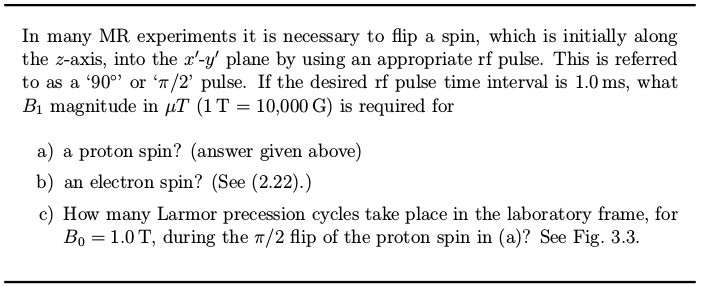
\includegraphics[width=0.8\textwidth,keepaspectratio]{prbl33}
    \label{fig:prbl33}
\end{figure}

\textit{Remember:}
\begin{itemize}
	\item For the same angle of tipping, the rf magnetic field will 
	depend on the type of particle (electron/proton). 
\end{itemize}

\textit{a) Proof.}
\begin{flalign*}
    \Delta \theta &= \gamma_p B_1 \tau \\
    \cancel{\pi} / 2\, \cancel{rad} &= 42.6 \times 10^6 \times 2\cancel{\pi}\, \cancel{rad}\, T^{-1} \cancel{s^{-1}}\, B_1\, 10^{-3} \cancel{s} \\
    B_1 &= \frac{1}{4 \times 42.6} \times 10^{-3}\, T \\ 
    B_1 &= 5.87 \mu T
\end{flalign*}

\textit{b) Proof.}
\begin{flalign*}
    \Delta \theta &= \gamma_e B_1 \tau \\
    \cancel{\pi} / 2\, \cancel{rad} &= 658 \times 42.6 \times 10^6 \times 2\cancel{\pi}\, \cancel{rad}\, T^{-1} \cancel{s^{-1}}\, B_1\, 10^{-3} \cancel{s} \\
    B_1 &= \frac{1}{4 \times 658 \times 42.6} \times 10^{-3}\, T \\ 
    B_1 &= 0.009 \mu T
\end{flalign*}

\textit{c) Proof.}
\begin{flalign*}
    \omega_0 &= \gamma B_0  \\
    \cancel{2\pi\, rad}\, \nu_0 &= 42.6 \times 10^6 \times \cancel{2\pi\, rad}\, \cancel{T^{-1}}\, s^{-1} \times 1\, \cancel{T}\\
    \nu_0 &= 42.6 \, MHz
\end{flalign*}


\clearpage
%%%%%%%%%%%%%%%%%%%%%%%%%%%%%%
\Large{Problem 3.4}
\begin{figure}[H]
    \centering
    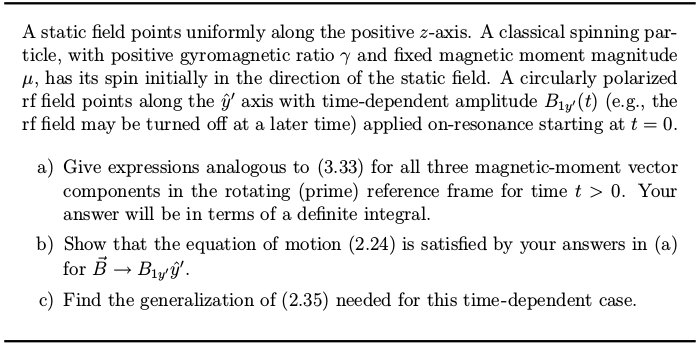
\includegraphics[width=0.8\textwidth,keepaspectratio]{prbl34}
    \label{fig:prbl34}
\end{figure}

\textit{Remember:}
\begin{itemize}
	\item The magnetic moment motion behaves similarly for an 
	on-resonance effective field.
\end{itemize}


\textit{a) You are asked to: } give solutions for the motion through time of the magnetic moment vector components when the $B_1$ field is a circularly polarised rf field pointing along the $\vec{y}'$ axis. \\
\textit{   Proof.}

\begin{figure}[H]
    \centering
    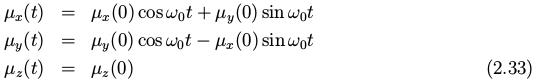
\includegraphics[width=0.7\textwidth,keepaspectratio]{form233}
    \label{fig:form233}
\end{figure}
The total effective field on-resonance will be given by $\vec{B} = B_{1y'}
\hat{y}'$. The magnetic moment vector motion is found by transcribing 
the solution (2.33) according to the substitutions: $z \rightarrow y', 
\, x \rightarrow z', \, y \rightarrow x' $ 
%(\frac{d\vec{\mu}}{dt})' &= \vec{\mu} \, \times [\hat{z}' (\omega_0 - \omega) + \hat{y}' \omega_1]  \\

\begin{flalign*}
    \mu_{x'}(t) &= \mu_{x'}(t_0) \, cos \, \phi_1(t) - \mu_{z'}(t_0) \, sin \, \phi_1(t) \\
    \mu_{y'}(t) &= \mu_{y'}(t_0) \\
    \mu_{z'}(t) &= \mu_{z'}(t_0) \, cos \, \phi_1(t) + \mu_{x'}(t_0) \, sin \, \phi_1(t)\\
    \text{with}: \\
    \phi_1 (t) &= \int_{t_0}^{t} dt' \omega_1(t') \\ 
    \text{in which}: \\
    \omega_1(t) &= \gamma \, B_1(t)
\end{flalign*}


\textit{b) Proof.}

\begin{figure}[H]
    \centering
    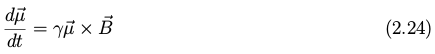
\includegraphics[width=0.6\textwidth,keepaspectratio]{form224}
    \label{fig:form224}
\end{figure}

\begin{flalign*}
    \vec{B}_{1y'}(t) &= B_{1y'} (t) \, \hat{y'} \\
	    			 &= B_{1y'} (t) \, (\hat{x} \, sin \omega t + \hat{y} \, cos \omega 
	    			 t) \\
	\text{We know that:} \\
	(\frac{d\vec{\mu}}{dt})' &= \gamma \vec{\mu}' \times \vec{B}_{1y'}  (t)
	\\
	\frac{d \mu_{x'}(t)}{dt} \hat{x}' + \frac{d \mu_{y'}(t)}{dt} 
	\hat{y}' + \frac{d \mu_{y'}(t)}{dt} \hat{z}' &= \gamma \, 
	(\mu_{x'}(t) \hat{x}' + \mu_{y'}(t) \hat{y}' + \mu_{z'}(t) 
	\hat{z}') \times B_{1y'} (t) \hat{y}' \\
	&= \gamma B_{1y'} (t) \, ( \mu_{x'}(t) \hat{x}' \times \hat{y}' + 
	\mu_{y'}(t) \hat{y}' \times \hat{y}' + \mu_{z'}(t) \hat{z}' \times 
	\hat{y}') \\
	&= \gamma B_{1y'} (t) \, ( \mu_{x'}(t) \hat{z}' - \mu_{z'}(t) \hat{x}' 
	)  \\
	\Rightarrow \\
	\frac{d \mu_{x'}(t)}{dt} &= - \gamma \mu_{z'}(t) B_{1y'} (t) = - 
	\omega_1 (t) \mu_{z'}(t) \\
	\frac{d \mu_{y'}(t)}{dt} &= 0 \\
	\frac{d \mu_{z'}(t)}{dt} &= \gamma \mu_{x'}(t) B_{1y'} (t) = 
	\omega_1 (t) \mu_{x'}(t)\\ \\
	\text{Taking the first derivative } & \text{of the solutions from 
	a) we get}: \\
	\frac{d \mu_{x'}(t)}{dt} &= - \, \mu_{x'}(t_0) \, \omega_1(t) \, sin \, 
	\phi_1(t) \, - \mu_{z'}(t_0) \, \omega_1(t) \, cos \, 
	\phi_1(t) \\
	&= - \, \omega_1(t) \, (\mu_{x'}(t_0) \, sin \, \phi_1(t) + \mu_{z'}(t_0) \, cos \, 
	\phi_1(t)) \\
	&= - \, \omega_1(t) \, \mu_{z'}(t) \\
	\frac{d \mu_{y'}(t)}{dt} &= 0 \\
	\frac{d \mu_{z'}(t)}{dt} &= - \, \mu_{z'}(t_0) \, \omega_1(t) \, sin \, 
	\phi_1(t) \, + \mu_{x'}(t_0) \, \omega_1(t) \, cos \, 
	\phi_1(t) \\
	&= \omega_1(t) \, (\mu_{x'}(t_0) \, cos \, \phi_1(t) - \mu_{z'}(t_0) 
	\, sin \, 
	\phi_1(t)) \\
	&= \omega_1(t) \, \mu_{x'}(t) \\
\end{flalign*}


\textit{c) Proof.}
\begin{figure}[H]
    \centering
    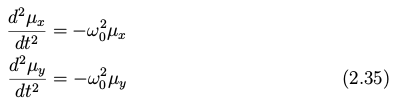
\includegraphics[width=0.6\textwidth,keepaspectratio]{form235}
    \label{fig:form235}
\end{figure}

\begin{flalign*}
	\frac{d^2 \mu_{x'}(t)}{dt^2} &= \frac{d}{dt} \, (\frac{d 
	\mu_{x'}(t)}{dt}) \\
    &= - \frac{d}{dt} \, (\omega_1(t) \mu_{z'}(t)) \\
    &= - \frac{d \omega_1(t)}{dt} \, \mu_{z'}(t) - \omega_1(t) \, \frac{d \mu_{z'}(t)}{dt}  \\
    &= - \frac{d \omega_1(t)}{dt} \, \mu_{z'}(t) - \omega_1^2(t) \mu_{x'}(t)  \\
	\frac{d^2 \mu_{z'}(t)}{dt^2} &= \frac{d}{dt} \, (\frac{d 
	\mu_{z'}(t)}{dt}) \\
	&= \frac{d}{dt} \, (\omega_1(t) \mu_{x'}(t)) \\
    &= \frac{d \omega_1(t)}{dt} \, \mu_{x'}(t) + \omega_1(t) \, \frac{d \mu_{x'}(t)}{dt}  \\
    &= \frac{d \omega_1(t)}{dt} \, \mu_{x'}(t) - \omega_1^2(t) \mu_{z'}(t) 
\end{flalign*}

\clearpage
%%%%%%%%%%%%%%%%%%%%%%%%%%%%%%
\Large{Problem 3.5}
\begin{figure}[H]
    \centering
    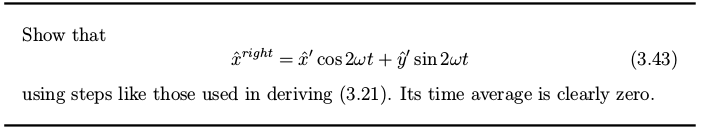
\includegraphics[width=0.8\textwidth,keepaspectratio]{prbl35}
    \label{fig:prbl35}
\end{figure}

\textit{Remember:}
\begin{itemize}
	\item A left-circularly polarized field is maximally effective in 
	tipping the spin around the $x'$-axis, while a right-circularly 
	polarized field is completely ineffective.
\end{itemize}

\textit{Proof.}\\
\textit{We know that:}
\begin{flalign*}
    \hat{x}^{right} &= \hat{x} \, cos \omega t + \hat{y} \, sin \omega t \\
    \hat{x}' &= \hat{x} \, cos \omega t - \hat{y} \, sin \omega t \\
    \hat{y}' &= \hat{x} \, sin \omega t + \hat{y} \, cos \omega t 
\end{flalign*}

\textit{Therefore, we can write:}
\begin{flalign*}
    \hat{x}' \, cos 2\omega t &= \hat{x} \, cos \omega t \, (1 - 2 sin^2 \omega t)  \\
                              &- \hat{y} \, sin \omega t \, (2 \, cos^2 \omega t - 1) \\
                              & = \hat{x} \, cos \omega t - 2 \hat{x} \, cos \omega t\, sin^2 \omega t  \\
                              &- 2 \hat{y}\, sin \omega t \, cos^2 \omega t + \hat{y}\, sin \omega t \\
    \hat{y}' \, sin 2\omega t &= 2 \hat{x} \, sin^2 \omega t\,cos \omega t \\
                              &+ 2 \hat{y}\,sin \omega t\, cos^2 \omega t
\end{flalign*}

\textit{By adding them together we get:}
\begin{flalign*}
    \hat{x}' \, cos 2\omega t + \hat{y}' \, sin 2\omega t &= \hat{x} \, cos \omega t + \hat{y}\, sin \omega t \Rightarrow\\
    \hat{x}' \, cos 2\omega t + \hat{y}' \, sin 2\omega t &= \hat{x}^{right}
\end{flalign*}

\textit{Calculating the time average:}
\begin{flalign*}
    <f(t)> &\equiv \frac{1}{T} \int_{0}^{T} f(t) dt \Rightarrow \\
\end{flalign*}
\begin{flalign*}
    <\hat{x}^{right} > &\equiv \frac{1}{T} \int_{0}^{T} \hat{x}' \, cos 
    2\omega t + \hat{y}' \, sin 2\omega t \, \, dt = \\
    &= \frac{1}{T} \int_{0}^{T} \hat{x} \, cos \omega t + \hat{y} \, sin 
    \omega t \, \, dt \\
\end{flalign*}
\begin{flalign*}
    &= \hat{x} \, \frac{1}{T} \int_{0}^{T} cos \, \omega t \, dt + 
    \hat{y} \, \frac{1}{T} \int_{0}^{T} sin \, \omega t \, dt \, 
    \Rightarrow \text{(as shown in \textit{Problem 3.2})} \\
    &= \mathbf{0}
\end{flalign*}


\clearpage
%%%%%%%%%%%%%%%%%%%%%%%%%%%%%%
\Large{Problem 3.6}
\begin{figure}[H]
    \centering
    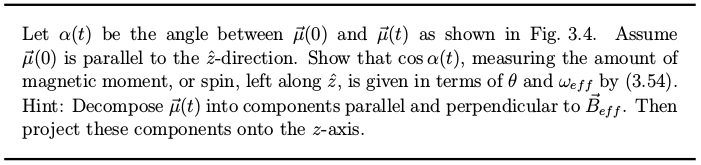
\includegraphics[width=0.8\textwidth,keepaspectratio]{prbl36}
    \label{fig:prbl36}
\end{figure}

\textit{Remember:}
\begin{itemize}
	\item The behaviour of the z-component of the magnetic moment is 
	shown here.
\end{itemize}

\begin{figure}[H]
        \centering
        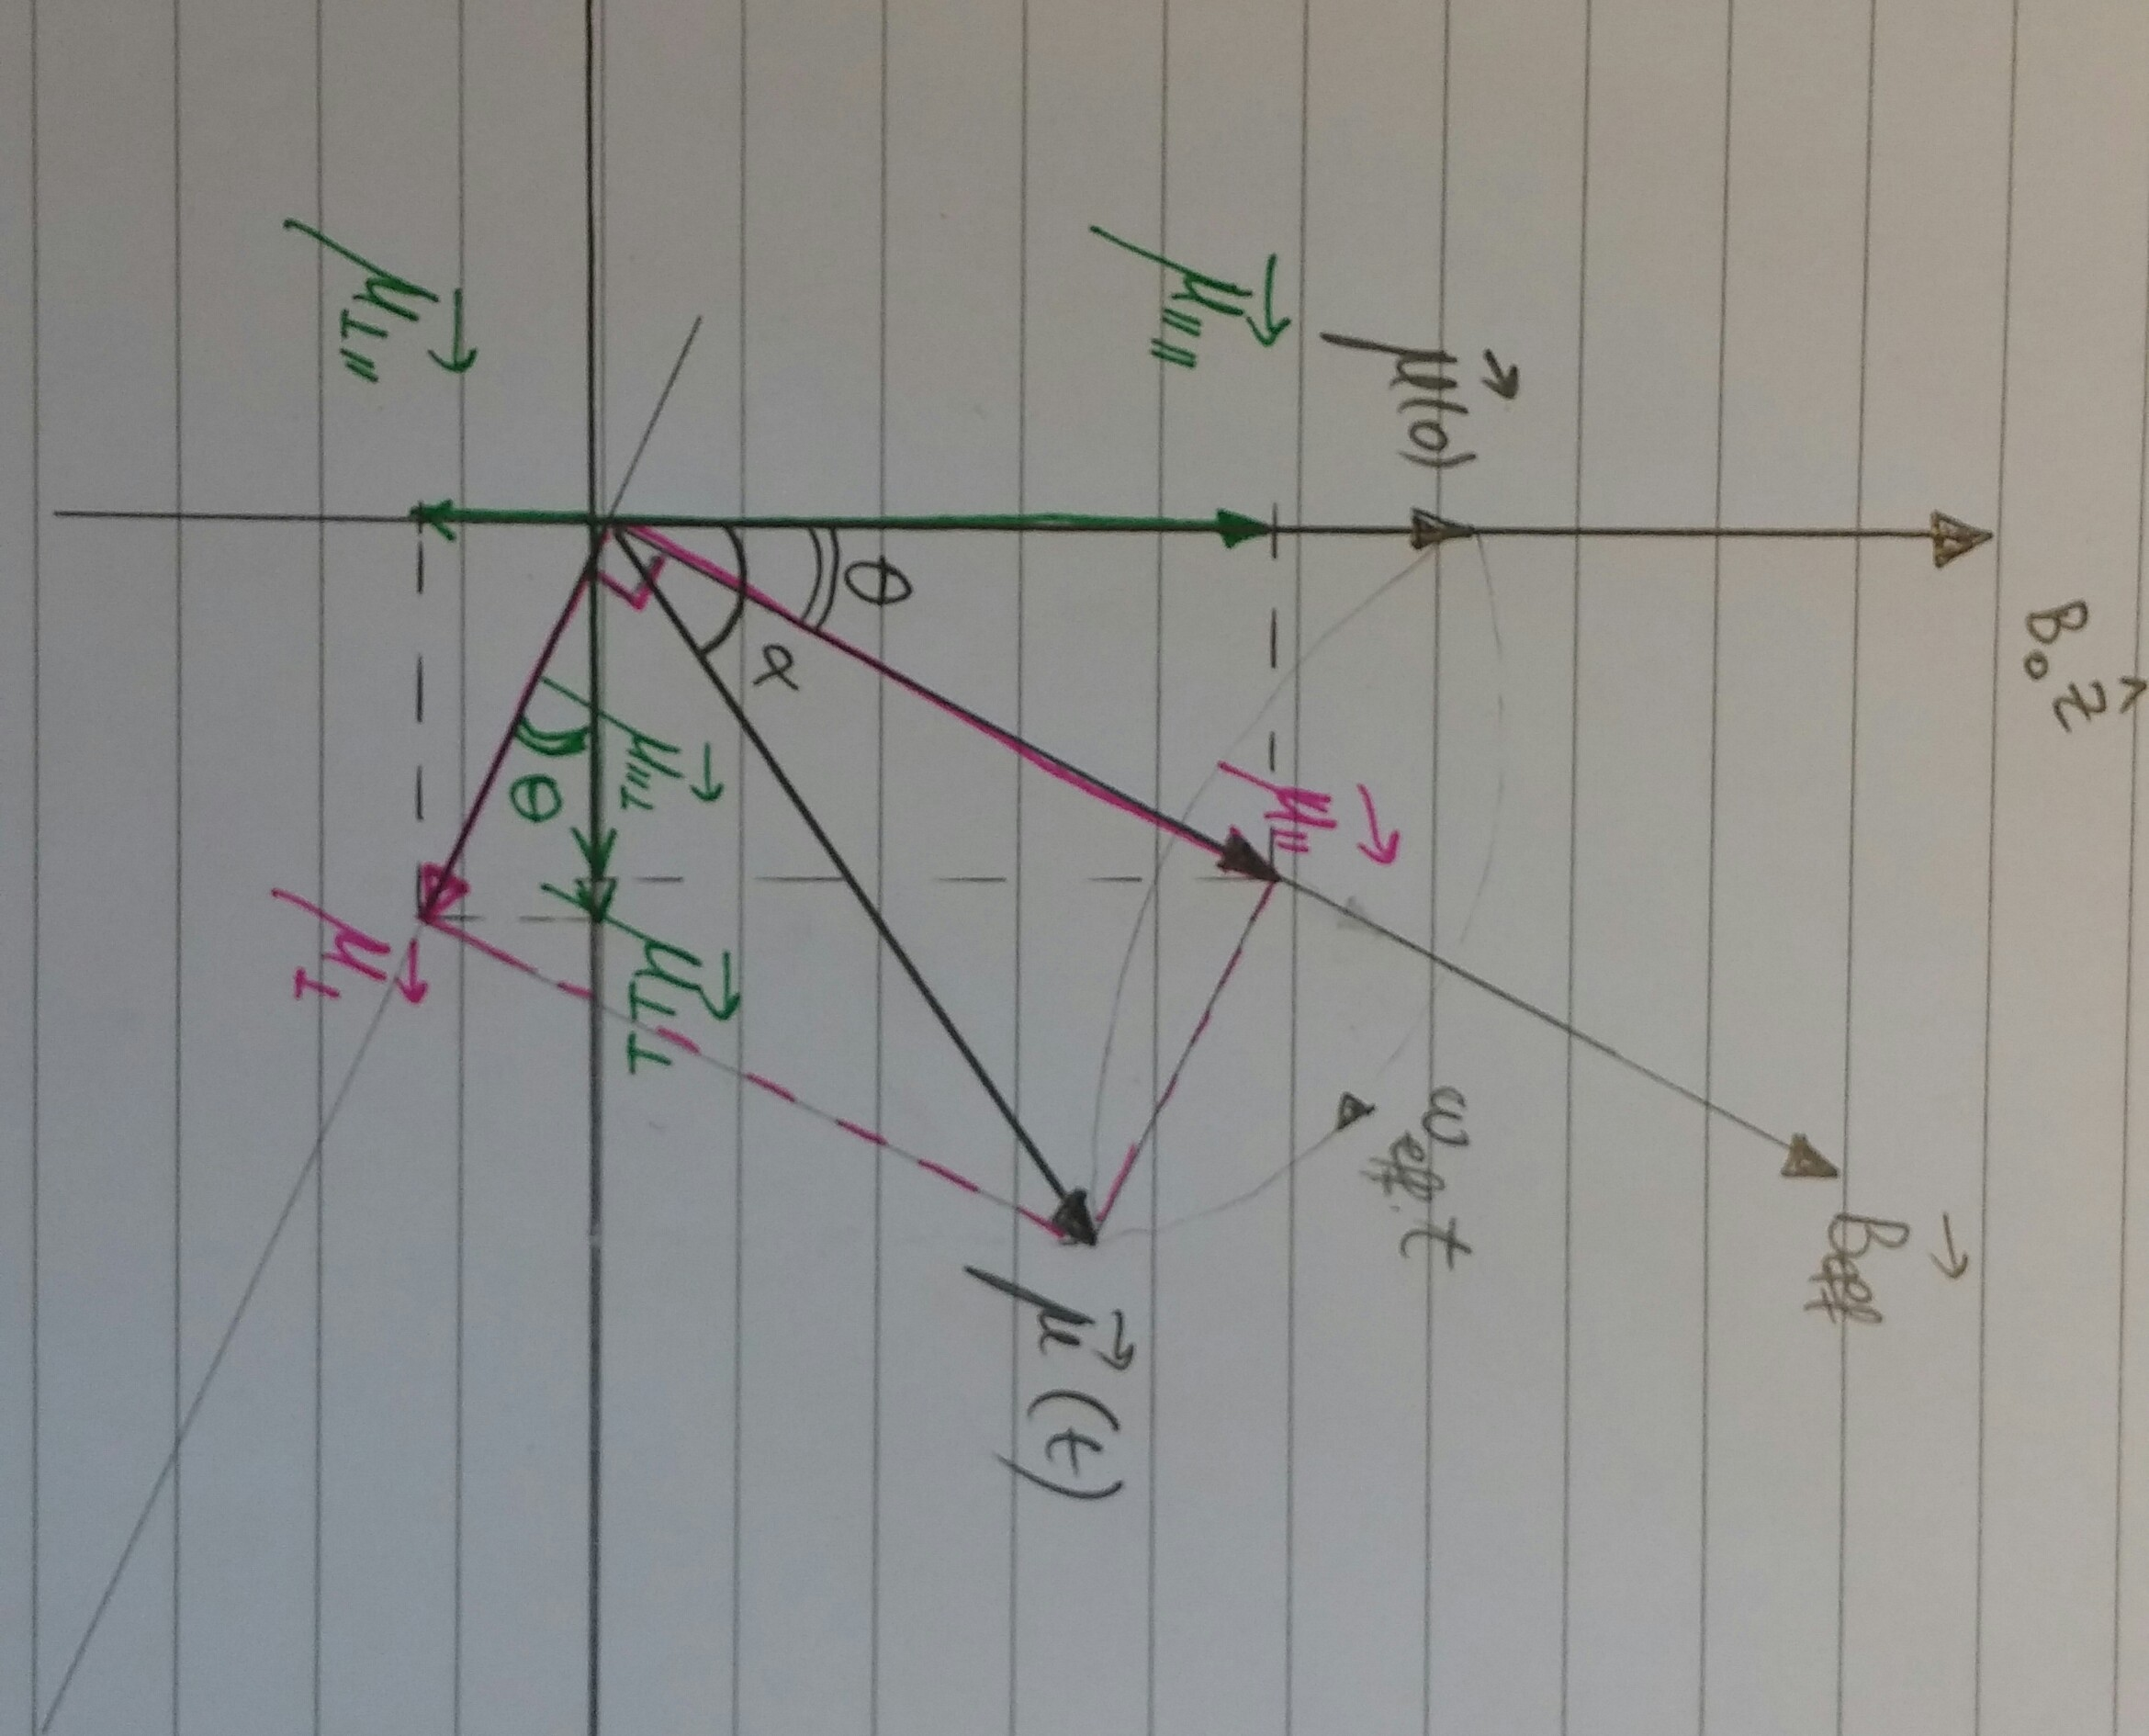
\includegraphics[angle=90,width=0.8\textwidth,keepaspectratio]{problem36}
        \label{fig:problem36}
\end{figure}

\textit{Proof.}



